\begin{align}
\vec{R} = \frac{\vec{Q} -2\vec{P}}{-1} 
= \myvec{3\\5},
\\
\frac{ (\vec{R} + \vec{Q})}{2}
=\myvec{2\\1} =\vec{P}.
\end{align}
See 
\figref{fig:chapters/12/10/5/9/Figure1}.
\begin{figure}[H]
	\begin{center}
		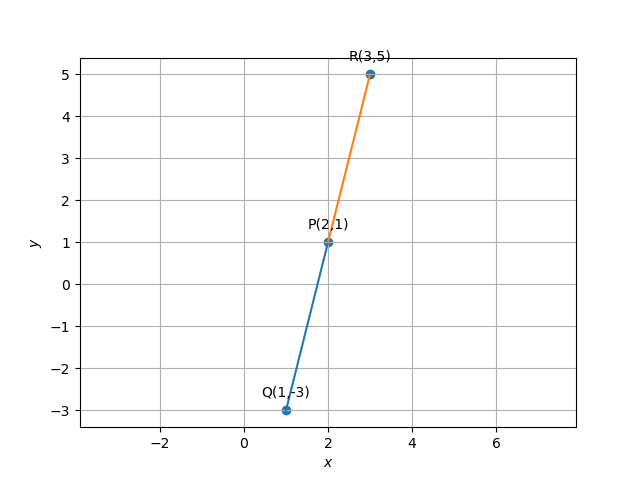
\includegraphics[width=0.75\columnwidth]{chapters/12/10/5/9/figs/line.png}
	\end{center}
\caption{}
\label{fig:chapters/12/10/5/9/Figure1}
\end{figure}
